\subsection{Stability}
As touched on in section \ref{sec:choice_of_cont}, the controller needs to be stable for the range in which the robot operates. The stability analysis will be preformed on the kinematic equation shown in \eqref{eq:base_system_eq2}. Since the robot has two controllers, for turning left and right, the kinematic function can be rewritten as.

\begin{equation}
    \Dot{\theta} = \frac{\Delta v}{2r_b} 
    \label{eq:stab1}
\end{equation}

\subsubsection{Continuous Time}

The $\Delta v$ will be seen as a constant and will be ignored in future equations. Using \eqref{eq:stab1}, the open-loop and closed-loop equation becomes.

\begin{equation}
    G_{ol}(s)=\frac{1}{2 r_b s}
\end{equation}

\begin{equation}
    G_{cl}(s)=\frac{G_{ol}(s)}{1+G_{ol}(s)}=\frac{(2r_b s)}{(2r_b s)*(2r_b s + 1)}
    \label{eq:stab12}
\end{equation}

\noindent The function \eqref{eq:stab12} has a pole and zero cancellation at origo. In Fig.\ref{fig:step1} the step response, poles and zeros are plotted for the closed loop system. Since all the poles appeare on the negative real plane, the system is stable.

\begin{figure}
    \centering
    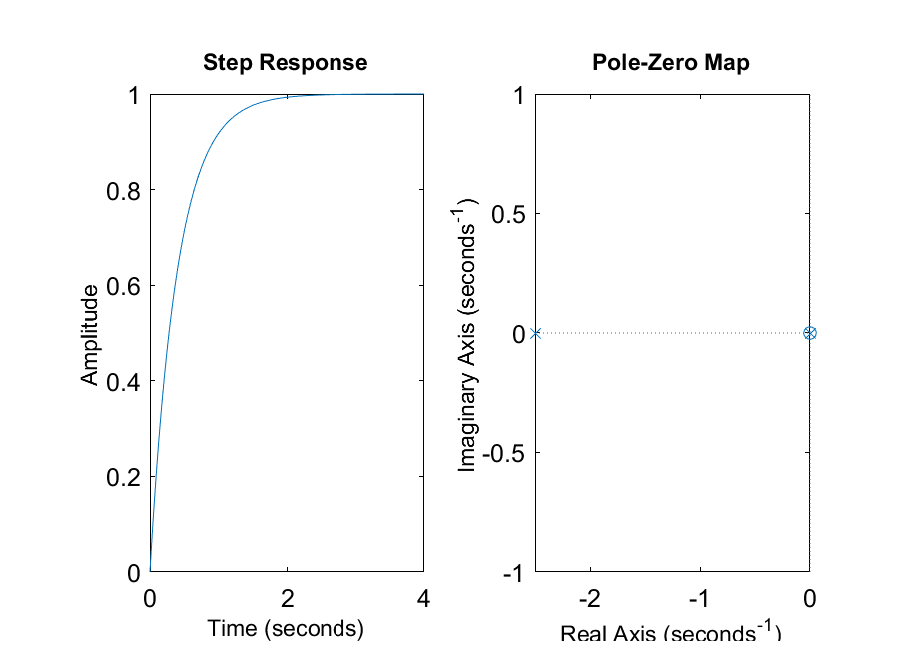
\includegraphics[width=0.7\textwidth]{img/closed_loop_step.eps}
    \caption{The closed loop system without a controller.}
    \label{fig:step1}
\end{figure}

\noindent The \textbf{PD}-controller discussed in previous sections only need to improve the system response, since the overall system is already stable. Introducing the controller to the system gives us the closed loop function.

\begin{equation}
    G_{clPD} = \frac{2r_b s(k_p + k_d s)}{2r_b s(s(2r_b+k_d)+k_p)}
\end{equation}

\noindent From this it's easy to see that the system will remain stables for $k_d > - 2 r_b$ and that the value of $k_d$ won't have any effect on the stability of the system in continuous time.\\
\indent The values for $k_p$ and $k_d$ is therefore chosen in such a manner that $ 0 > k_d > -2 r_b$ and $k_p$ so that the greatest error input from the \textbf{MV}-node will not saturate the actuators. The result of these are shown in Fig.\ref{fig:step2} and a comparison was made, represented in table \ref{tab:with_without}.

\begin{figure}[H]
    \centering
    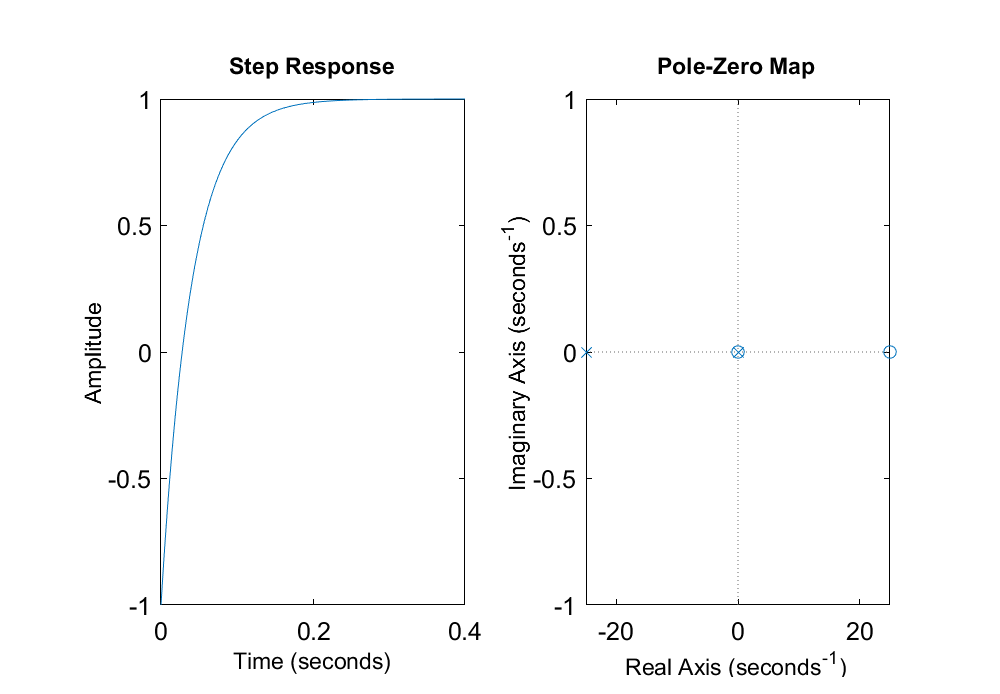
\includegraphics[width= 0.7\textwidth]{img/closed_loop_step_PD.eps}
    \caption{The closed loop system with a controller.}
    \label{fig:step2}
\end{figure}

\begin{table}[H]
    \centering
    \caption{Comparison between the closed loop systems.}
    \begin{tabular}{|c|ccc|}
        \hline & Without controller & \textbf{PD}-controller & Discrete Time \textbf{PD}-controller \\
        \hline Rise Time & 0.8788$s$ & 0.0879$s$ & 0.1000$s$ \\ 
        Settling Time & 1.5648$s$ & 0.1565$s$ & 0.2500$s$ \\
        \hline
    \end{tabular}
    \label{tab:with_without}
\end{table}


\subsubsection{Discrete Time}
Using MATLAB to move from continuous time to discrete time with a update frequency of 20 Hz\footnote{The update frequency of the camera} and an input delay of $1/30s$\footnote{Estimated input delay to the actuators}. In Fig.\ref{fig:stepD} it's clear that the pole is within the unit circle on the discrete time plane and that the responds follows the step input. In conclusion, the system is stable using the $k_p$ and $k_d$ values proposed above, even in discrete time \cite{torkel_ljung}.

\begin{figure}[H]
    \centering
    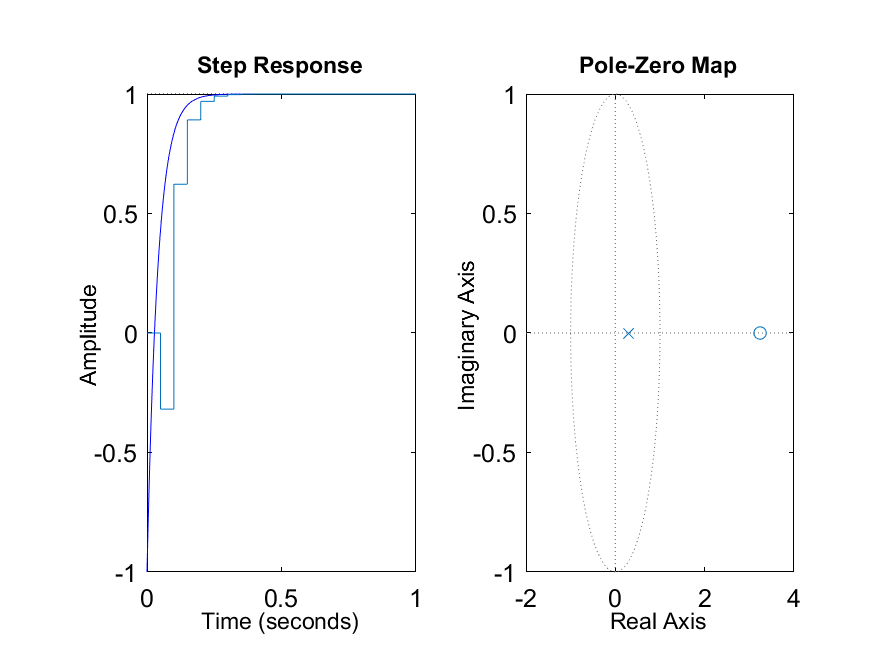
\includegraphics[width= 0.7\textwidth]{img/closed_loop_step_D.eps}
    \caption{The continuous step response, discrete step response and the poles and zeros of the discrete transfer function.}
    \label{fig:stepD}
\end{figure}
